%3D Pythagoras - Cuboid


\documentclass[tikz,border=10pt]{standalone}
\usepackage{tikz}
\usetikzlibrary{3d} % for 3d vector calculations

\begin{document}

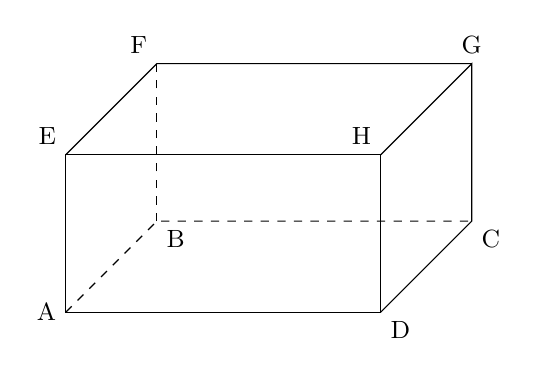
\begin{tikzpicture}[scale=1, transform shape]
    % Define the points of the cube
    \coordinate (A) at (0,0,0);
    \coordinate (B) at (0,0,-3);
    \coordinate (C) at (4,0,-3);
    \coordinate (D) at (4,0,0);
    \coordinate (E) at (0,2,0);
    \coordinate (F) at (0,2,-3);
    \coordinate (G) at (4,2,-3);
    \coordinate (H) at (4,2,0);

    % Draw the visible edges of the cube
    \draw (A) -- (D) -- (H) -- (E) -- cycle; % bottom face
    \draw (D) -- (C) -- (G) -- (H); % right face
    \draw (E) -- (F) -- (G); % top face

    % Draw the hidden edges of the cube
    \draw[dashed] (A) -- (B) -- (C);
    \draw[dashed] (B) -- (F);

    % Place the labels with smaller font size
    \node at (A) [left,font=\small] {A};
    \node at (B) [below right,font=\small] {B};
    \node at (C) [below right,font=\small] {C};
    \node at (D) [below right,font=\small] {D};
    \node at (E) [above left,font=\small] {E};
    \node at (F) [above left,font=\small] {F};
    \node at (G) [above,font=\small] {G};
    \node at (H) [above left, font=\small] {H};
\end{tikzpicture}

\end{document}